\section{Эксперимент}
\label{sec:Chapter5} \index{Chapter5}

\subsection{Описание эксперимента}

%Постановка эксперимента. Что планируется сделать и какие результаты хочется получить. Какие метрики будем использовать и по каким метрикам будем сравнивать.

В рамках данного исследования было решено провести эксперимент по адаптации моделей распознавания ключевых точек на теле человека к целевому набору данных. В представленном разделе будет рассказано про выбранные модели, алгоритм доменной адаптации, описание исходного и целевого наборов данных и метрик оценивания результатов работы нейронных сетей.

\subsubsection*{Выбор модели для эксперимента}

Многие модели из представленных в \autoref{sec:Chapter4} были представлены в рамках проекта MMPose, что значительно облегчило эксперимент с точки зрения подготовки пайплайнов предобработки данных и построения конфигураций нейронных сетей. Также критерием отбора стала возможность обучения модели в условиях ограниченных вычислительных ресурсов, так как адаптация проводилась в рамках платформы Google Colab.

\begin{table}[H]
	\centering
	\begin{center}
	\begin{tabular}{
	|>{\centering\arraybackslash}m{4cm}
	||>{\centering\arraybackslash}m{3cm}
	|>{\centering\arraybackslash}m{3cm}
	|>{\centering\arraybackslash}m{4cm}|}
		\hline
		\centering Название модели&Количество параметров&Размер входящего изображения&Время предсказания\\
		\hline
		\hline
		HRNet & 28,5 M & $256 \times 192$ & 203,7 мс\\
		\hline
		ViTPose & 90 M & $256 \times 192$ & 269,8 мс\\
		\hline
		SimCC + Resnet  & 36,8 M & $256 \times 192$ & 101 мс\\
		\hline
		RTMPose  & 13 M & $256 \times 192$ & 55,4 мс\\
		\hline
	\end{tabular}
	\end{center}
	\caption{Характеристики моделей, выбранных для эксперимента.}
	\label{tab:models}
\end{table}

В итоге было выбрано 4 модели, описание которых представлено в \autoref{tab:models}. Они будут обучены на исходном домене в течении 20 эпох. От этого состояния будет начинать при проведении адаптации.

\subsubsection*{Описание метода доменной адаптации}

В рамках эксперимента будет оптимизирован метод Progressive Unsupervised Learning \cite{pul} для задачи распознавания ключевых точек. 

Основной сложностью выступает выбор функции фильтрации невалидных результатов. И в рамках эксперимента предлагается использовать фильтрацию по уровню уверенности модели в предсказанной ключевой точке. Средняя уверенность полученных из предсказания результатов для одного изображения будет сравниваться с заранее заданным пороговым значением. Все значения, перешедшие этот порог попадают в псевдо-обучающую выборку.

Заметим, что для точек, которые не являются видимыми, уверенность сильно меньше, что может портить среднюю уверенность для фотографии. Таким образом получаем ещё одну функцию фильтрации - по средней уверенности для видимых точек результата.

На каждой итерации будет проводиться дообучение модели в течение 10 эпох. Количество итераций будет ограничено либо сходимостью метрики качества, либо количеством 10 штук.

\subsubsection*{Метрики оценки качества распознавания}

Для проведения количественной оценки работы алгоритма во всех случаях необходимо использовать метрики оценки предсказания. Выбранные метрики дают полную оценку того, насколько хорошо модель работает, как с точки равнозначности всех точек в топологии, так и с учетом их веса в скелете.\\

\begin{enumerate}
\item \textit{Percentage of Correct Keypoints}

Первой рассмотрим метрику PCK, которая равнозначно воспринимает все ключевые точки. Для нее важно попало ли предсказания в окрестности реального результата, причем размер окрестности может быть выбран как фиксированный для всего тестового набора, так и зависеть от высоты человека на изображении. 

Математическую формулу метрики можно представить в следующем виде:

\begin{equation}
	PCK = \frac{\sum_{i=1}^{n} bool(d_i < threshold * body\_height)}{n},
\end{equation}
	
где $d_i$ - расстояние между предсказанной и правильной точкой,\\
$threshold$ - порог, задаваемый исследователем,\\
$body\_height$ - высота прямоугольника, внутри которого находится человек,\\
$bool(*)$ - логическое условие, возвращает 1, если оно верно и 0 в ином случае,\\
$n$ - размер выборки.

\item \textit{Object Keypoint Similarity}

OKS была представлена для оценки решений задачи распознавания ключевых точек в рамках соревнования COCO \cite{COCO_topology}. Авторы старались провести аналогию с метрикой Intersection over Union (IoU) для задачи детекции объектов, чтобы можно было пользоваться метрикой average precision, о которой будет рассказано далее.

В отличие от предыдущей метрики, OKS не считает все точки равнозначными. Для этого проводится процедура нормализации расстояния между предсказанной и реальной точками. Одним из шагов нормализации является учет размера детектируемого объекта, что показывает различия для детекции скелета людей на заднем и переднем планах. Вторым шагом нормализации является учет дисперсии данной ключевой точки.

Математическая формула метрики выглядит следующим образом:

\begin{equation}
	OKS = \frac{\sum_{i} exp\left( - d_i^2 / 2s^2k_i^2\right)\delta\left(v_i > 0\right)}{\sum_{i} \delta\left(v_i > 0\right)},
\end{equation}

где $d_i$ - расстояние между предсказанной и правильной точкой,\\
$s$ - масштаб объекта,\\
$k_i$ - константа ключевой точки, контролирующая спад,\\
$v_i$ - видимость точки по аннотации COCO, где 0 обозначает, что точка не была размечена.

\item Average Precision

AP - метрика, широкоиспользуемая для оценки качества моделей в задача классификации и обнаружения объектов. Она измеряет точность нейронной сети, принимая во внимание как ее способность правильно классифицировать объекты, так и ее способность точно их локализовать.

Исходя из названия метрика использует такие понятие как Precision, показывающее доли правильно предсказанных положительных примеров среди всех положительно предсказанных результатов, и Recall, показывающее долю правильно предсказанных положительных примеров среди всех фактических положительных примеров.
$$
Precision = \frac{TP}{TP + FP} \text{, } Recall = \frac{TP}{TP + FN}
$$
При использовании OKS верно положительным результатом является тот, для которого метрика OKS больше заданного порогового значения. Неверно положительными являются те результаты, метрика OKS для которых не перешла заранее заданный порог. Неверно отрицательными являются все реальные данные, для которых результата получено не было.
$$
TP\text{ при }OKS > threshold\text{ и }FP\text{ при }OKS \leq threshold
$$
Используя описанные пояснения можно рассчитать значения метрик точность и полнота. С их помощью строится кривая precision-recall, которая показывает изменения точности в зависимости от полноты. Площадь под ее графиком и будет являться значением метрики AP. Часто она высчитывается интегрирования кривой precision-recall методом трапеций, который показан на \autoref{fig:trapz}.

\begin{figure}[h]
	\centering
	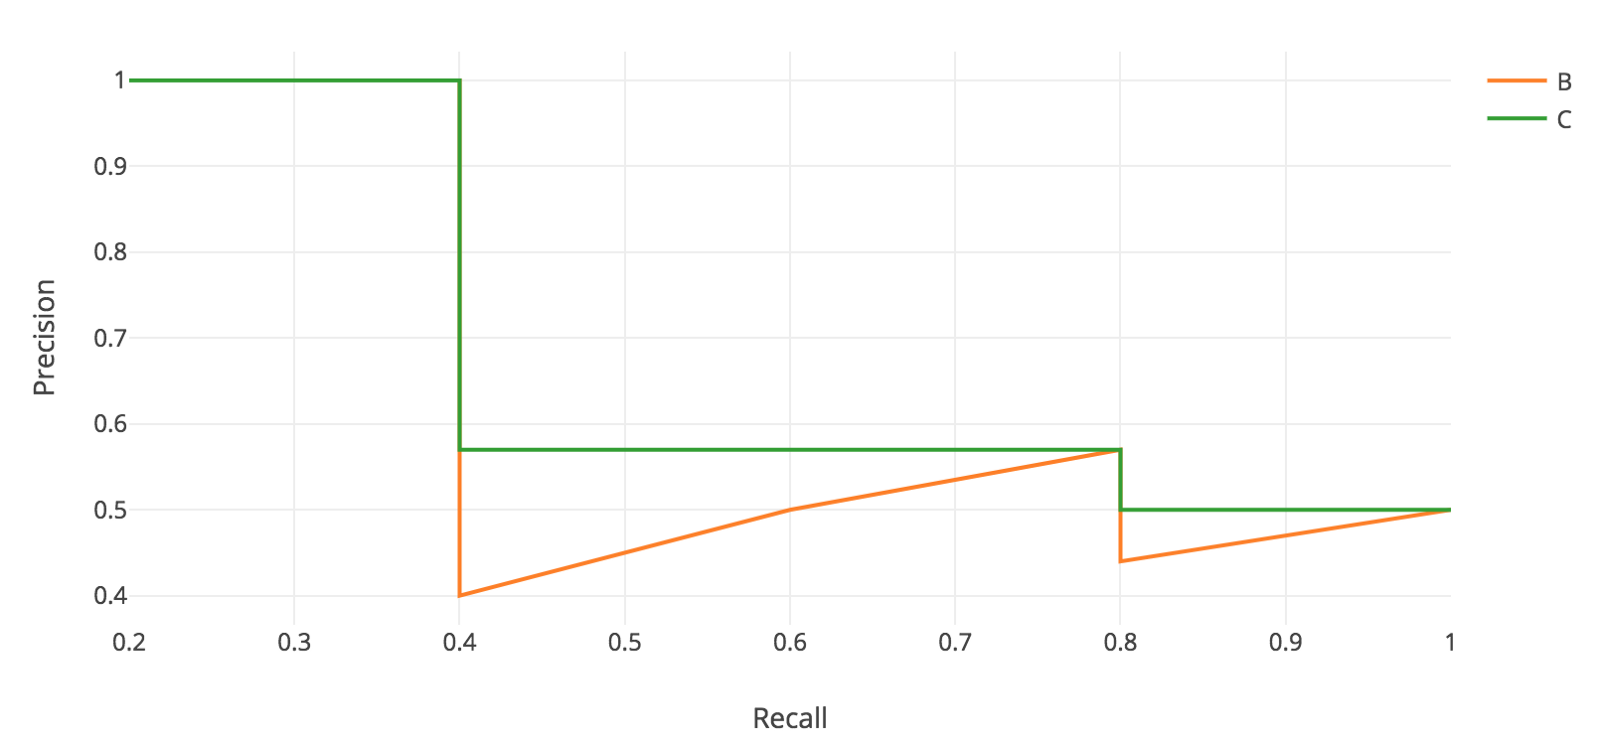
\includegraphics[width=.75\textwidth]{./images/AP}
	\caption{Применения метода трапеций для интегрирования кривой precision-recall.}
	\label{fig:trapz}
\end{figure}

Для задачи детекции обычно применяется несколько порогов: $AP^{0.5}$, $AP^{0.75}$ и $AP = mAP = mean AP^{0.5:0.05:0.95}$.

\end{enumerate}

\subsection{Данные}

По условиям задачи доменной адаптации необходимо найти два набора данных для эксперимента. Далее приведем информацию о выбранных доменах и их характеристиках.

\subsubsection*{Исходный домен}

В качестве исходного домена выбран набор данных Common Objects in Context \cite{COCO_dataset}. COCO — это крупный датасет, широко используемый в области компьютерного зрения для задач распознавания объектов, сегментации, и создания описательных подписей к изображениям. Он был создан Microsoft и с тех пор стал стандартом для обучения и оценки алгоритмов компьютерного зрения.

\begin{figure}[h]
	\centering
	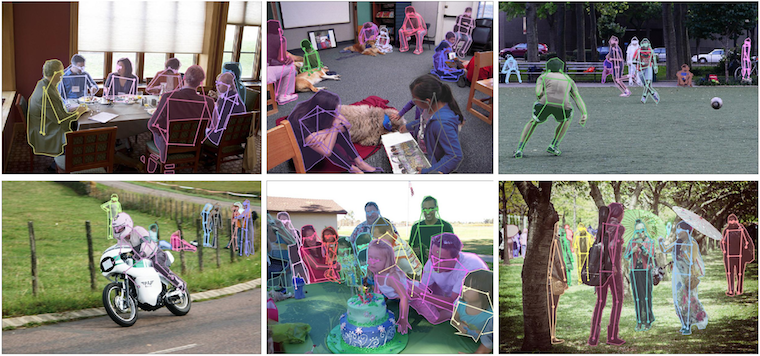
\includegraphics[width=\textwidth]{./images/data_info/coco_dataset}
	\caption{Примеры изображений из набора данных COCO. \cite{COCO_topology}}
	\label{fig:coco_dataset}
\end{figure}

Учитывая, что в рамках соревнований COCO была и задача детекции ключевых точек (Keypoint detection) \cite{COCO_topology}, то часть этого набора данных была размечена под нее. Если быть точным, то датасет включает более 250 тысяч аннотаций людей на различных изображениях. Формат аннотаций включает в себя:

\begin{enumerate}

\item \textit{id} - уникальный номер аннотации;

\item \textit{image\_id} - уникальный номер изображения, которому принадлежит данная аннотация;

\item \textit{category\_id} - уникальный номер категории, к которой относится данная аннотация. Для задачи оценки позы везде выставляется категория person;

\item \textit{keypoints} - массив из 17 ключевых точек, для каждой их которых указаны координаты (x, y) на изображении, а также информация о видимости. Точки, которые не представлены на изображении заполняются нулями;

\item \textit{num\_keypoints} - здесь содержится информация о количестве размеченных точек для данной аннотации;

\item \textit{bbox} - информация об ограничивающем человека прямоугольнике. Значения внутри лежат в следующем формате: $[x, y, width, height]$;

\item \textit{area} площадь сегментированного человека. Значение необходимо при высчитывании метрики OKS;

\item \textit{iscrowd} - информация о том, одиночный человек представлен на изображении или толпа людей.

\end{enumerate}

Также в рамках задачи Keypoint Detection была введена метрика OKS и метрика mAP, о которых было рассказано ранее. Они представляют собой единые критерии для оценки моделей, что облегчает сравнение и улучшение результатов различных алгоритмов, поэтому регулярно используются для оценки  новых методов и технологий.

В рамках задачи были выбраны 8000 аннотаций, которые содержат все 17 ключевых точек то топологии COCO. На них и было произведено обучение моделей для получения бейзлайнов эксперимента.

\subsubsection*{Целевой домен}

%Описание собранных данных. Численный объем датасета. Возможно количество локаций и распределение по ним.

%Необходимо предоставить данные по распределению данных между людьми, по количеству данных для обучения/тестирования. Предоставить данные по локациям. Предоставить картинки с примерами данных, которые были собраны.

%Описание системы полуавтоматической разметки данных. Что там использовалось и как проходит разметка.

В качестве целевого набора данных был собран отдельный набор данных боксеров. В наборе данных представлены 2 человека, снятые с 3 ракурсов: профиль, анфас и 3/4. Датасет состоит из 10 видеозаписей, которые содержат порядка 10 тысяч кадров. Для проведения эксперимента выбрано 2,6 тысячи изображений, которые были впоследствие размечены. Из них для тестовой выборки отобрано около 420 изображений, а оставшиеся 2200 составили обучающую выборку, на которой и проводилась адаптация.

\begin{figure}[h]
\begin{subfigure}[b]{0.24\textwidth}
	\centering
	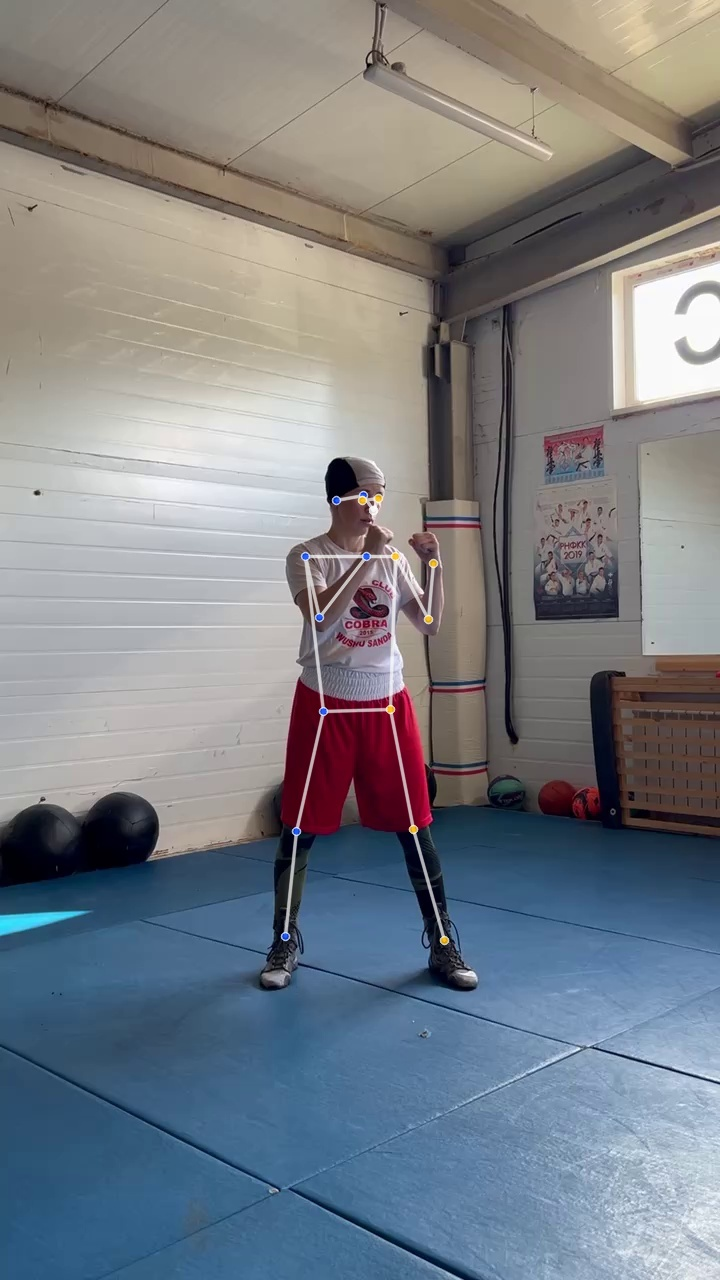
\includegraphics[width=\textwidth]{./images/data_info/box_examples/ex_5}
\end{subfigure}
\begin{subfigure}[b]{0.24\textwidth}
	\centering
	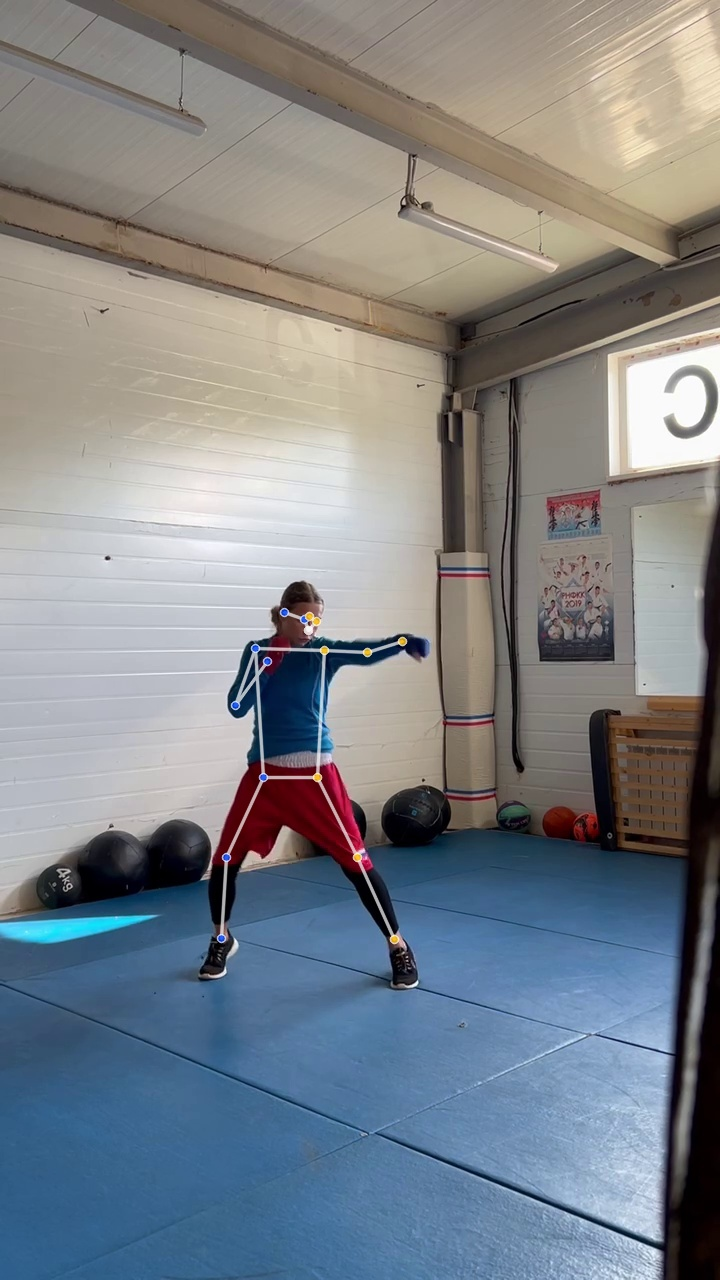
\includegraphics[width=\textwidth]{./images/data_info/box_examples/ex_1}
\end{subfigure}
\begin{subfigure}[b]{0.24\textwidth}
	\centering
	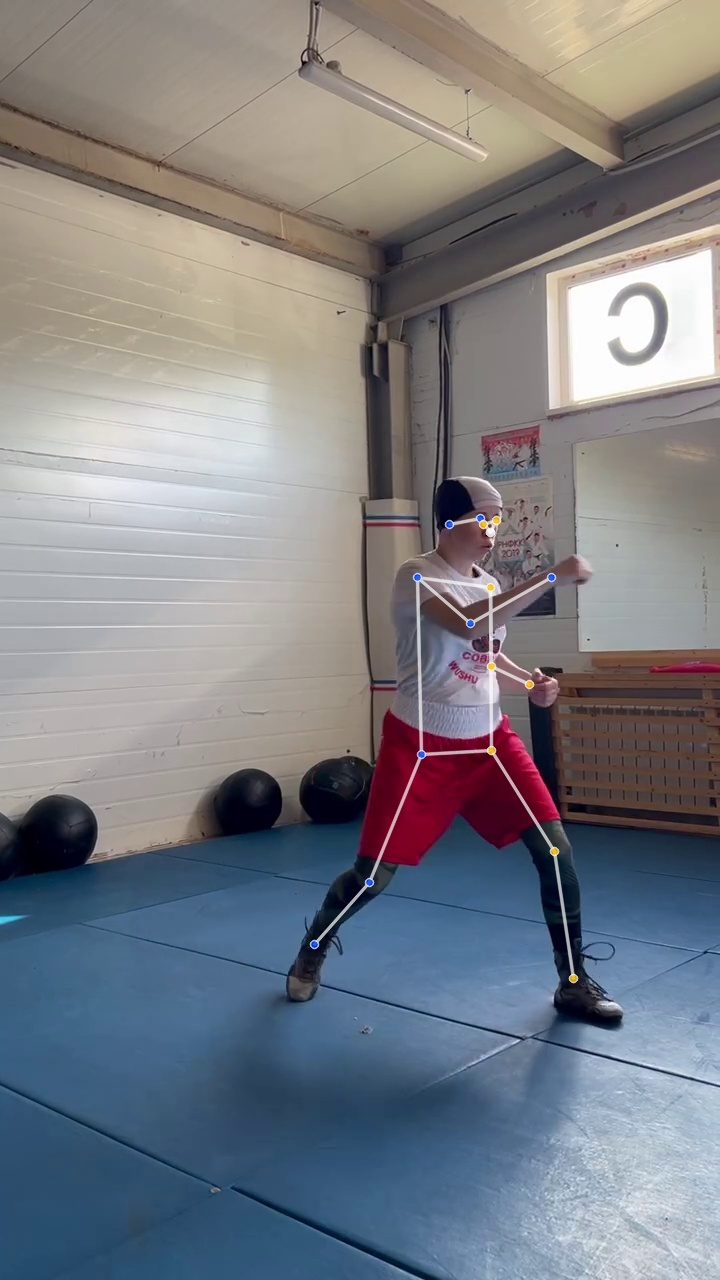
\includegraphics[width=\textwidth]{./images/data_info/box_examples/ex_9}
\end{subfigure}
\begin{subfigure}[b]{0.24\textwidth}
	\centering
	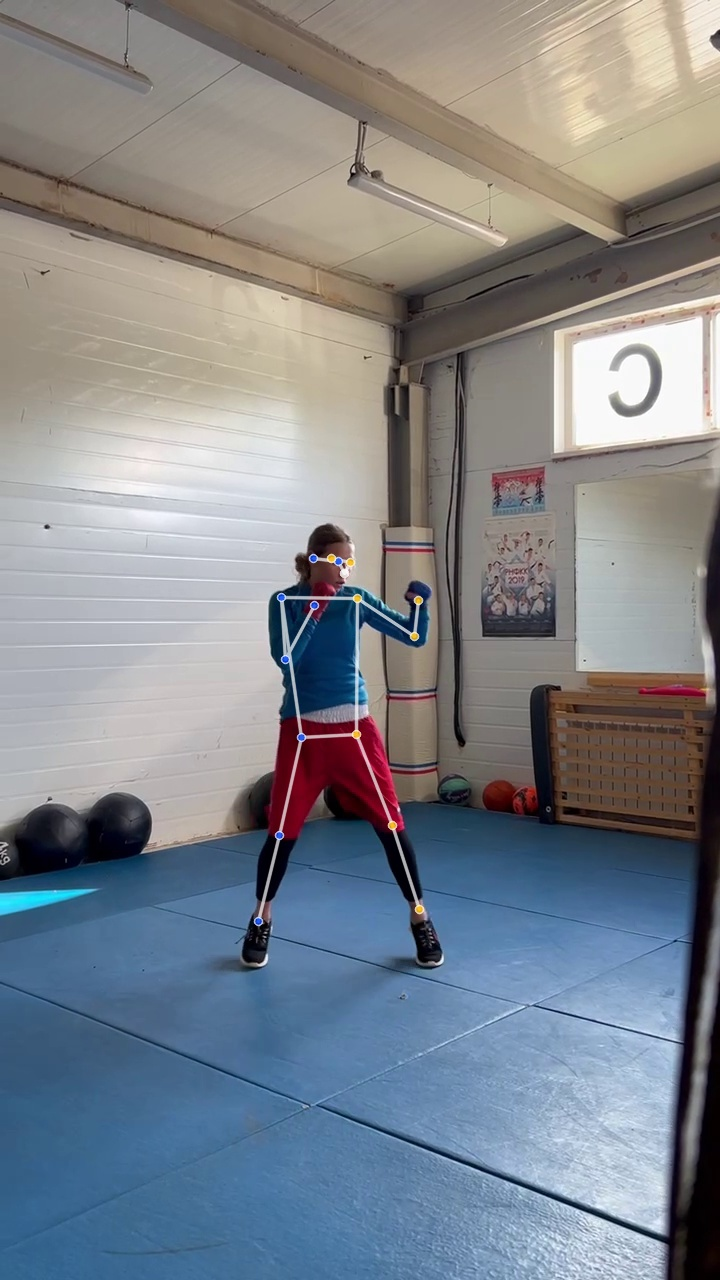
\includegraphics[width=\textwidth]{./images/data_info/box_examples/ex_0}
\end{subfigure}
\caption{Примеры изображений целевого домена.}
\label{fig:target_examples}
\end{figure}

В рамках задачи по аннотированию собранных данных была разработана система полуавтоматической разметки изображений pose-markup \cite{pose_markup}. Она представляет собой предобученную модель распознавания ключевых точек и инструмент для визуальной корректировки данных экспертом.

Для автоматической части использовалась модель BlazePose от проекта MediaPipe \cite{mediapipe}. Выбор сделан благодаря высоким характеристикам скорости инференса результатов и их точности у данного решения. А также для того, чтобы избежать корреляции размеченных данных с предсказаниями, которые будут оцениваться в рамках эксперимента. Результат, возвращаемый моделью был преобразован к формату аннотаций COCO, который был описан выше и сохранен в формате JSON. 

\begin{figure}[h]
\begin{subfigure}[b]{0.32\textwidth}
	\centering
	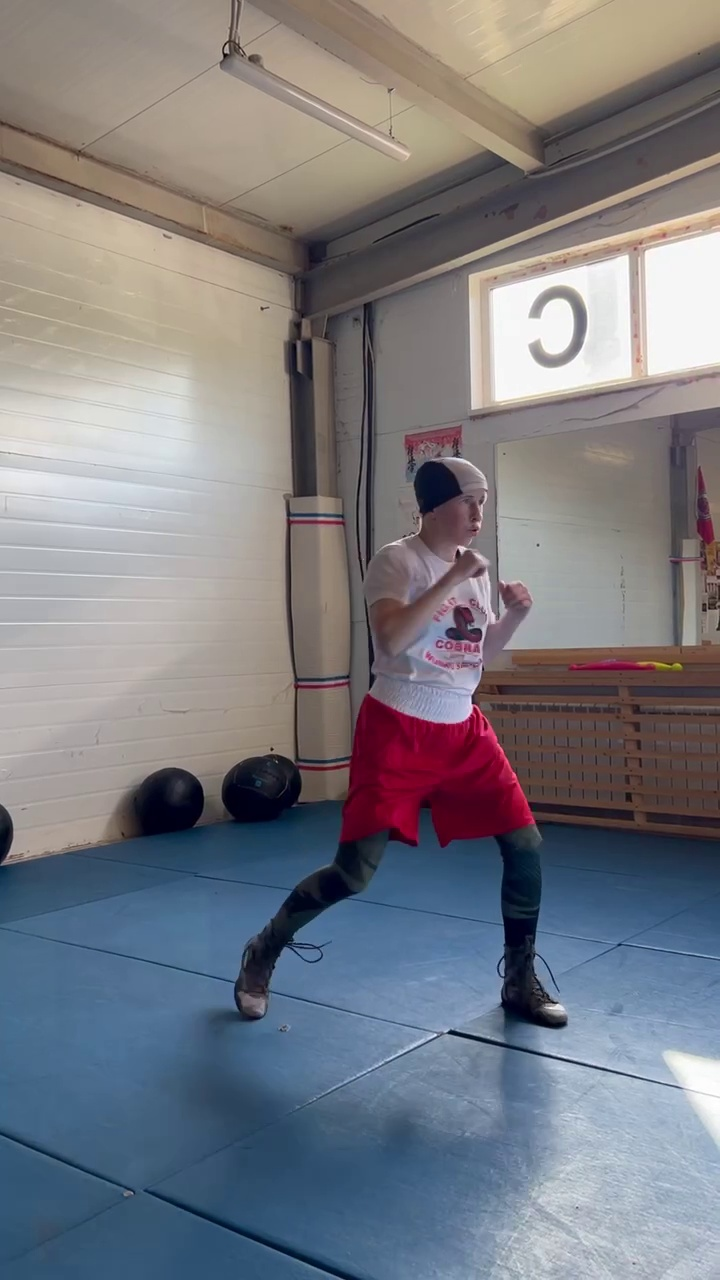
\includegraphics[width=\textwidth]{./images/data_info/pose_markup_examples/raw}
	\caption{Изначальное изображение}
\end{subfigure}
\begin{subfigure}[b]{0.32\textwidth}
	\centering
	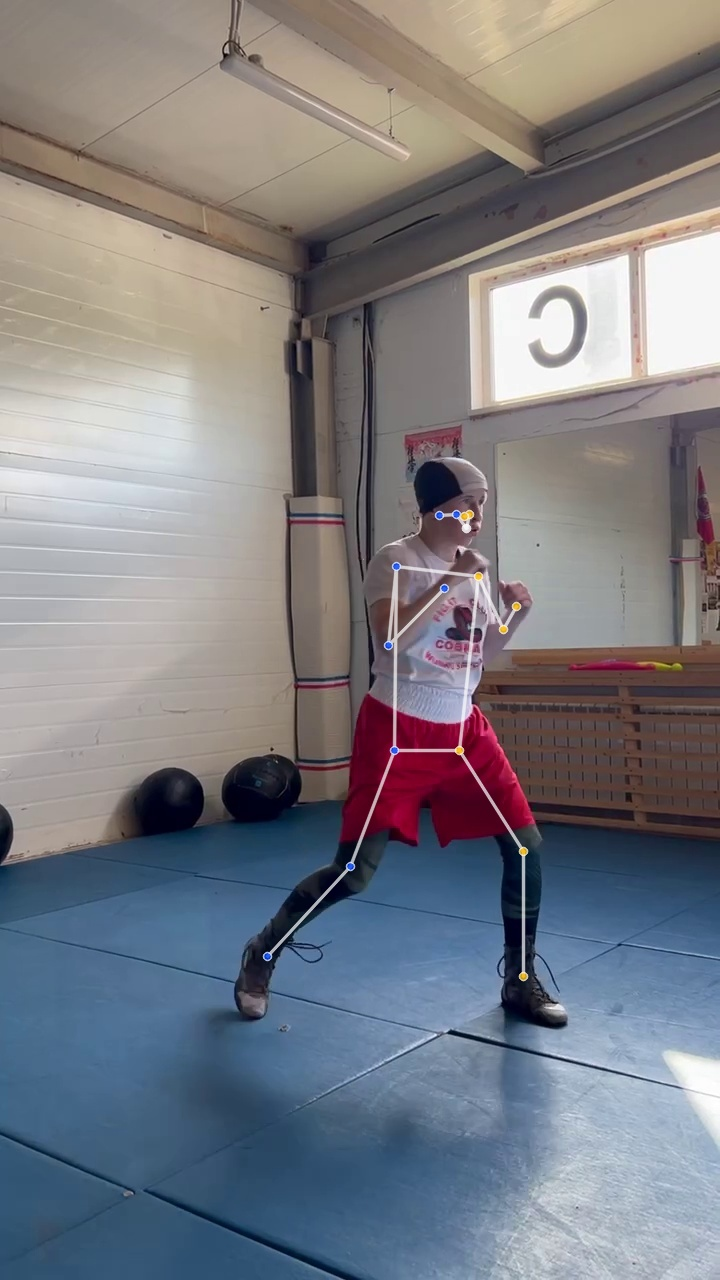
\includegraphics[width=\textwidth]{./images/data_info/pose_markup_examples/auto_labeled}
	\caption{После автоматической разметки}
\end{subfigure}
\begin{subfigure}[b]{0.32\textwidth}
	\centering
	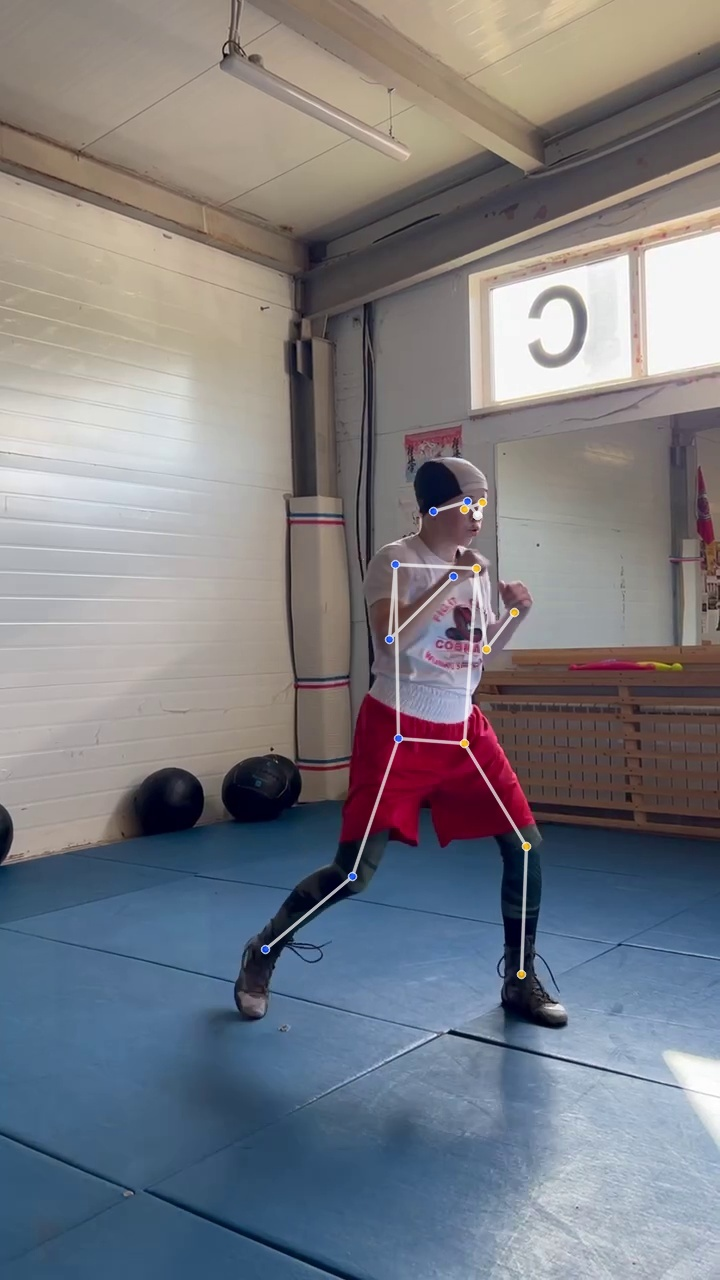
\includegraphics[width=\textwidth]{./images/data_info/pose_markup_examples/correct_labels}
	\caption{После корректировки экспертом}
\end{subfigure}
\caption{Пример работы системы полуавтоматической разметки данных.}
\label{fig:pose_markup_example}
\end{figure}

Как можно видеть на \autoref{fig:pose_markup_example}, модель имеет неточности, которые необходимо было исправить эксперту. Для этой цели использовалась вторая часть программы - инструмент для визуальной корректировки данных экспертом. 

Проанализировав результаты внесенных изменений, получили, что каждый кадр требовал правки ключевых точек. Средние показатели изменений на кадр:

\begin{itemize}
\item Собирая статистику любых изменений в точках, даже сдвига на соседний пиксель, получаем, что в среднем 14.9 точек на кадре были изменены. Распределение этих исправлений по топологии представлено на \autoref{fig:any_correction}.
\item Если считать точки, которые были значительно сдвинуты (5 и более пикселей), то их в среднем приходилось 6.5 на кадр. Большинство из них были сосредоточены на лице и левой конечности человека. Более детальное распределение изменений по топологии представлено на \autoref{fig:big_correction}.
\end{itemize}

\begin{figure}[h]
\centering
\begin{subfigure}[b]{0.4\textwidth}
	\centering
	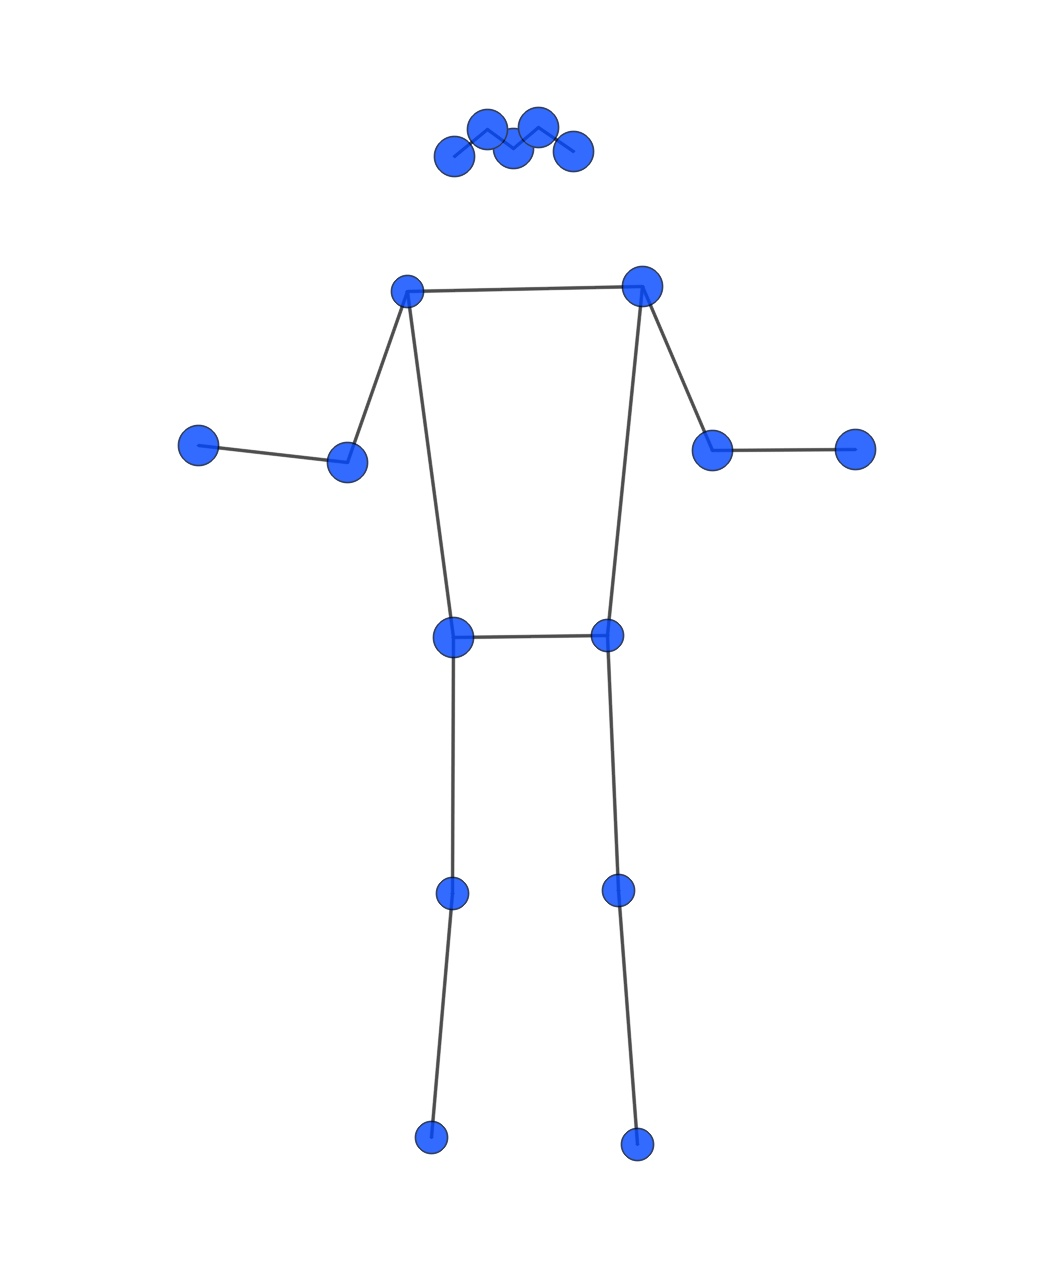
\includegraphics[width=\textwidth]{./images/data_info/pose_markup_examples/change_percentage}
	\caption{}
	\label{fig:any_correction}
\end{subfigure}
\begin{subfigure}[b]{0.4\textwidth}
	\centering
	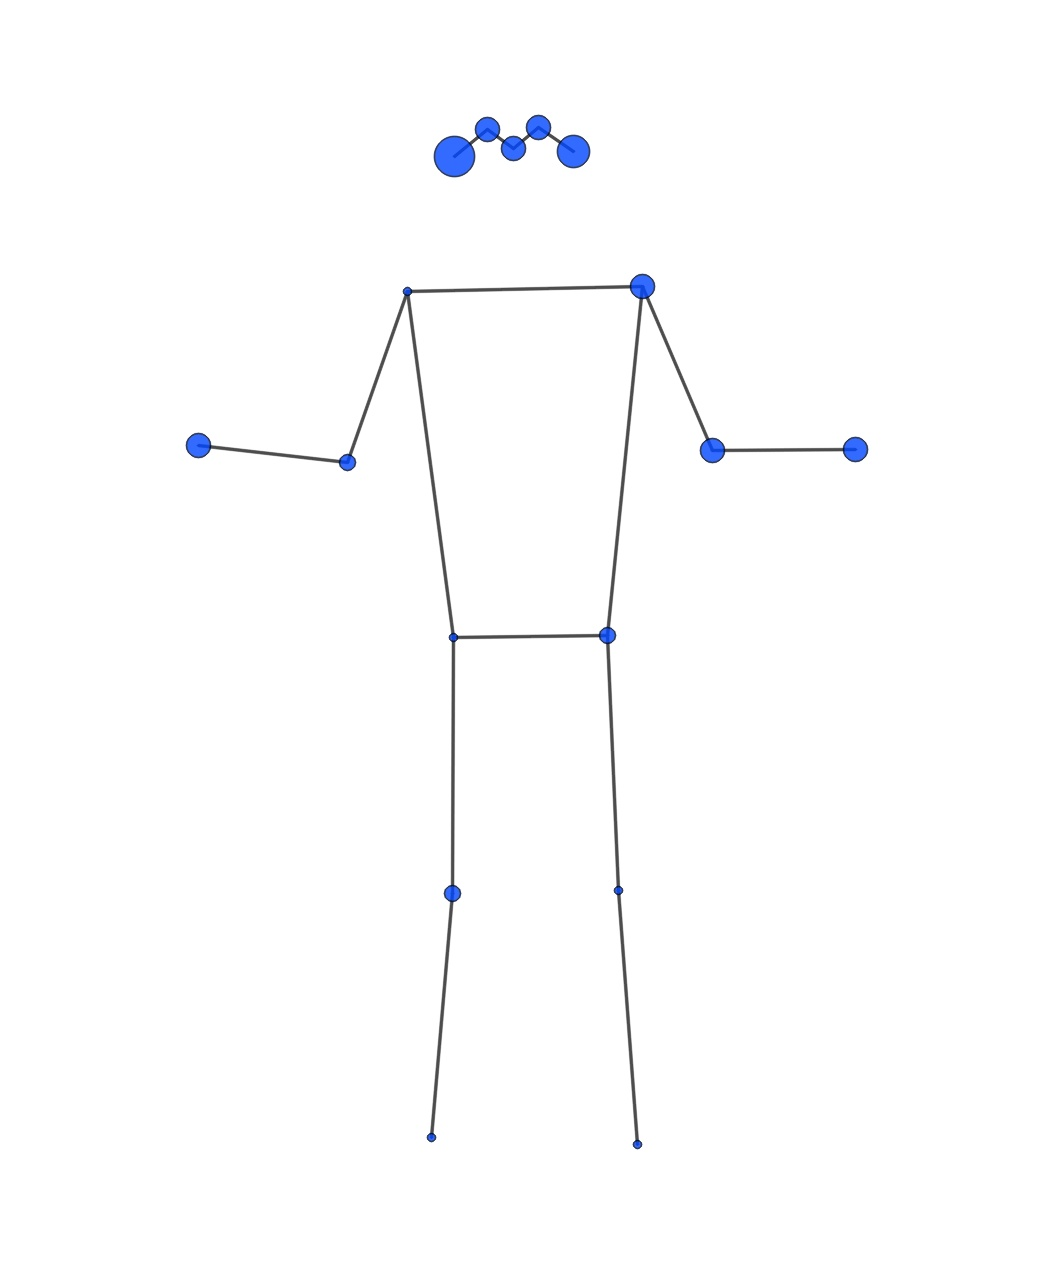
\includegraphics[width=\textwidth]{./images/data_info/pose_markup_examples/big_change_percentage}
	\caption{}
	\label{fig:big_correction}
\end{subfigure}
\caption{Схематическое представление изменений в точках, внесенных экспертом.}
\label{fig:correction_heatmap}
\end{figure}

\subsection{Результаты эксперимента}

%Тут можно сказать про ресурсы и про то, какие постановки эксперимента будут сделаны.

%Предоставить относительно сухо результаты эксперимента. Можно дать базовый анализ ситуации и того, что мы видим.

%Необходимо предоставить результаты по времени обучения нейросетей, времени дообучения нейросетей. 
%Собрать данные по количеству ошибок до-после обучения. Собрать данные по количеству ошибок при изменении домена. 
%Данные по ресурсам, на которых обучались нейросетки.


В рамках эксперимента для выбранных ранее моделей был применен алгоритм доменной адаптации PUL, который показал смешанные результаты на разных архитектурах. В качестве функции фильтрации было выбрано отсеивание результатов предсказания поз на основе средней уверенности в предсказанных точках. Порог уверенности для каждой модели выбирался исходя из результатов первых итераций алгоритма. Так как на первых из них уверенность модели в своих результатах падала из-за внесения обучения на псевдо-данных. Влияние фактора подбора порога будет оценено далее.

 адаптированная модель сравнивается с базовыми весами, которые обучены на исходном домене, а также с дообученной на размеченных целевых данных. Это позволит оценить полезность и применимость работы алгоритма доменной адаптации.

Тестирование моделей производилось с использованием графического ускорителя NVIDIA MX250 с 2 Гб памяти. Так как объемов памяти этого ускорителя не хватало для обучения моделей, для обучения моделей была соверешена миграция в облачный сервис Google Colab с использованием предоставляемого там графического ускорителя NVIDIA Tesla T4 с 16 Гб памяти.

\subsubsection*{HRNet}

В рамках первого эксперимента использовалась архитектура HRNet. Так как уверенность на бейзлайне не была высокой, то пришлось выставить порог уверенности в 0.4. В связи с этим для итеративных процессов отбирались данные, которые не являются точными и вносят большую ошибку. Это стало причиной того, что с каждой итерацией модель показывала все более плохие результаты, которые можно увидеть на \autoref{fig:hrnet_pck}.

\begin{figure}[h]
	\centering
	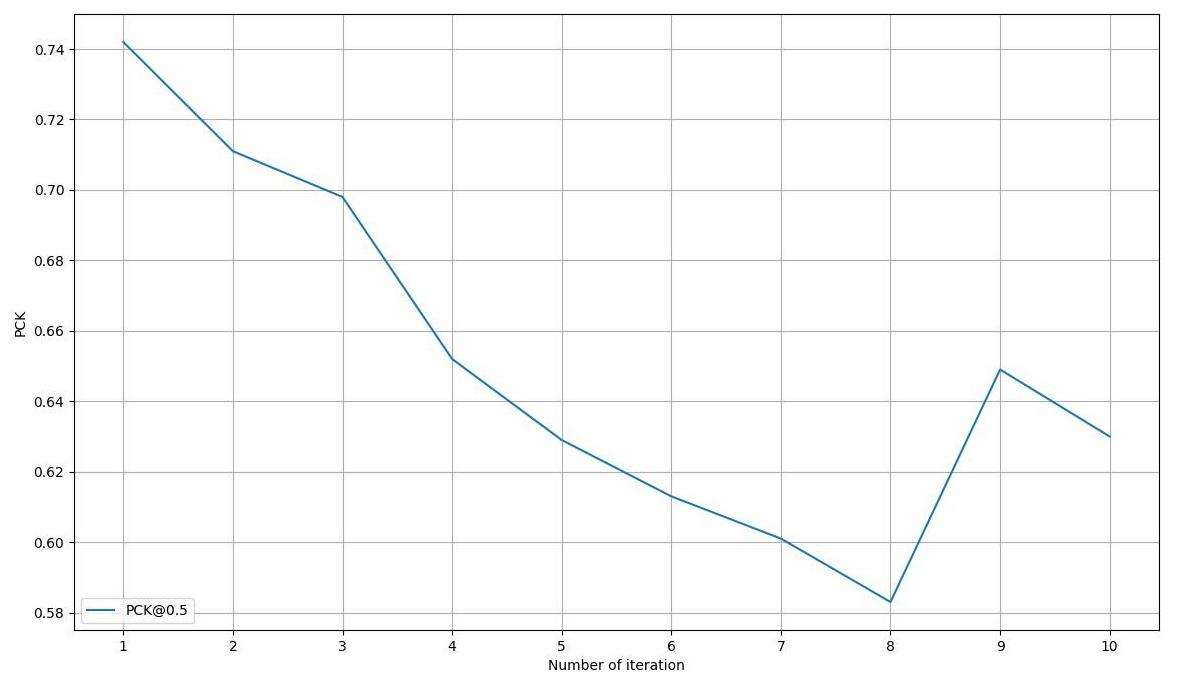
\includegraphics[width=.9\textwidth]{./images/results/hrnet/hrnet_pck}
	\caption{Зависимость метрики PCK на целевом домене от номера итерации.}
	\label{fig:hrnet_pck}
\end{figure}

Остальные результаты для данной модели не снимались в виду плохих результатов адаптации. В дальнейшем значение порога будет выбираться не ниже 0.5.

\subsubsection*{ViTPose}

Исходя из опыта предыдущего эксперимета, порог уверенности был выбран равным 0.7. Особенностью данного эксперимента явилось то, что модель быстро достигла высокой уверенности в своих результатах, из-за чего объемы псевдо-разметок были равными объему всей выборки для адаптации. Из \autoref{fig:vitpose_pck} видно, что итеративный процесс можно было остановить на 4 этапе, что могло сэкономить время эксперимента. Это состояние и будет считаться адаптированным в рамках данного эксперимента.

\begin{figure}[H]
	\centering
	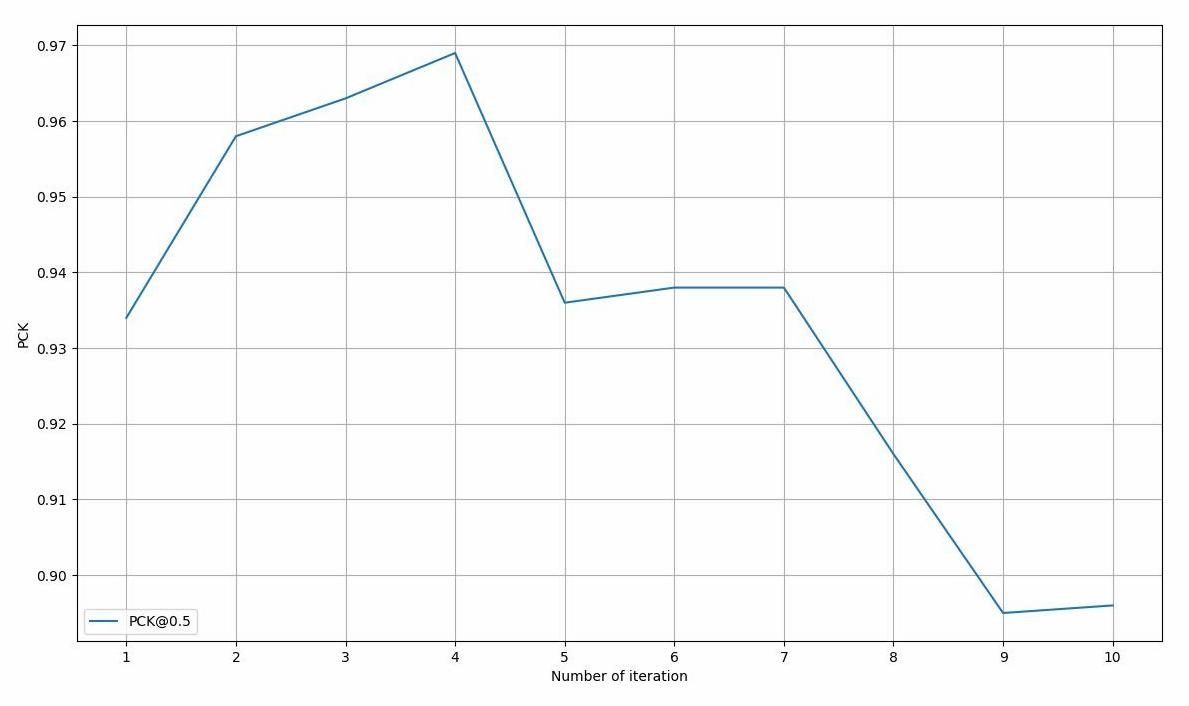
\includegraphics[width=\textwidth]{./images/results/vitpose/vitpose_pck}
	\caption{Зависимость метрики PCK на целевом домене от номера итерации для модели ViTPose.}
	\label{fig:vitpose_pck}
\end{figure}

Метрики, снятые на разных версиях модели, показаны в \autoref{tab:vitpose_table}. Можно заметить, что адаптированная модель предсказывает больше точек, по сравнению с другими моделями, но точность предсказания показывает значительно более плохие результаты. 

\begin{table}[H]
	\centering
	\begin{tabular}{
	|p{3.3cm}
	||>{\centering\arraybackslash}p{2.2cm}
	|>{\centering\arraybackslash}p{2.2cm}
	|>{\centering\arraybackslash}p{2cm}|}
		\hline
		&PCK@0.05&PCK@0.25&PCK@0.5\\\hline
		\hline
		Baseline & 0.147 & 0.725 & 0.902 \\
		\hline
		Adapted model & 0.118 & 0.623 & 0.969 \\
		\hline
		Finetune model  & 0.21 & 0.789 & 0.948 \\
		\hline
	\end{tabular}
	\begin{tabular}{
	|p{3.3cm}
	||>{\centering\arraybackslash}p{4cm}
	|>{\centering\arraybackslash}p{4.6cm}|}
		\hline
		&Время обучения&Время предсказания\\\hline
		\hline
		Baseline & 118 мин & 250,2 мс\\
		\hline
		Adapted model & 10 мин & 248,3 мс\\
		\hline
		Finetune model  & 30,5 мин & 246,5 мс\\
		\hline
	\end{tabular}
	\caption{Сравнительная статистика нескольких состояний модели ViTPose.}
	\label{tab:vitpose_table}
\end{table}

На \autoref{fig:vitpose_distr} показано распределение адаптированной метрики PCK применительно ко всем точкам топологии в отдельности. Как можно заметить на \autoref{fig:vitpose_distr_05}, у базового состояния возникли проблемы с точками внешних конечностей, но и дообучение, и адаптация улучшили их предсказание. Но при уменьшении радиуса допустимой ошибки, мы наблюдаем на \autoref{fig:vitpose_distr_025}, что адаптированная модель показывает хорошие результаты только для точек нижних конечностей. Причем точность предсказания точек головы ухудшается для обоих попыток изменения модели. 

\begin{figure}[H]
\centering
\begin{subfigure}{.8\textwidth}
	\centering
	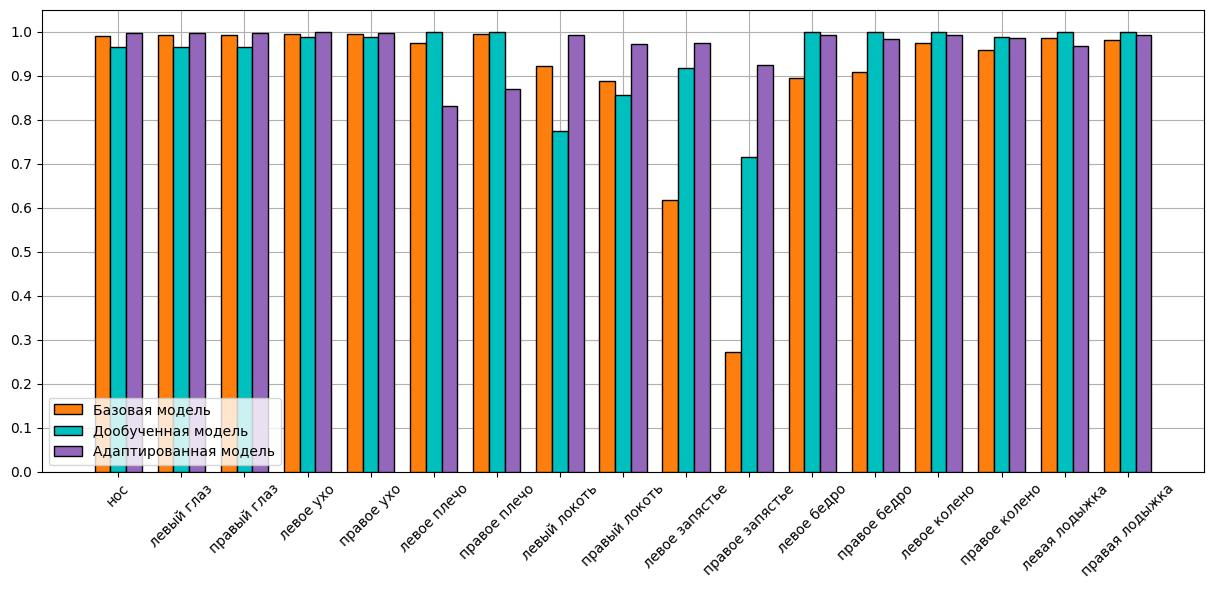
\includegraphics[width=\textwidth]{./images/results/vitpose/vitpose_05_s}
	\caption{Аналог PCK@0.5}
	\label{fig:vitpose_distr_05}
\end{subfigure}
\begin{subfigure}{.8\textwidth}
	\centering
	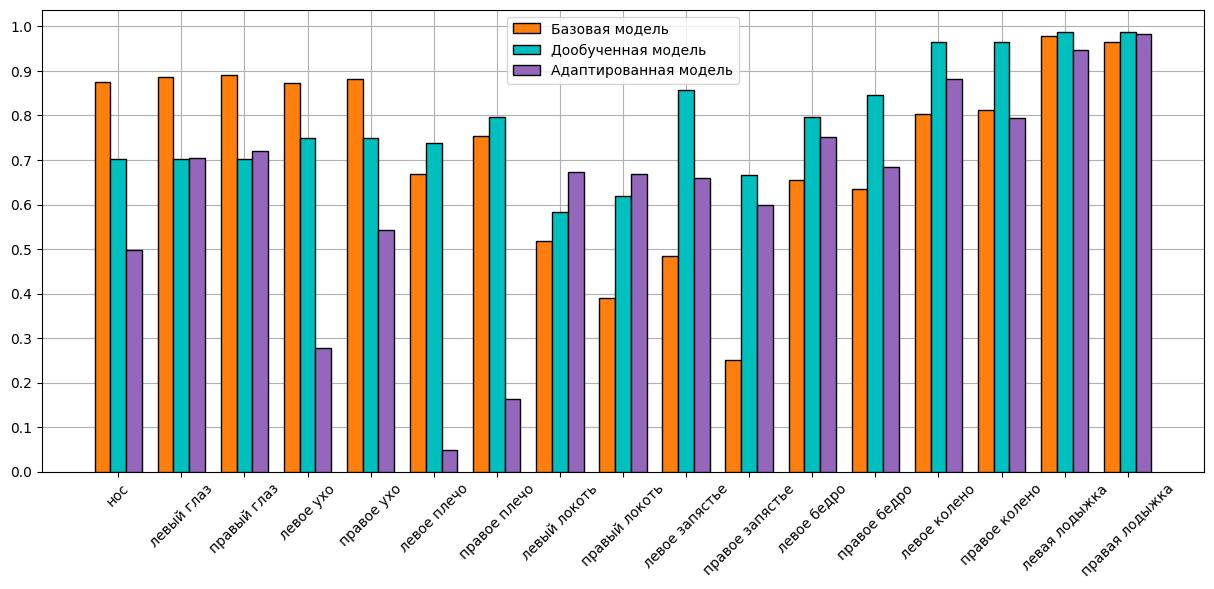
\includegraphics[width=\textwidth]{./images/results/vitpose/vitpose_025_s}
	\caption{Аналог PCK@0.25}
	\label{fig:vitpose_distr_025}
\end{subfigure}
\caption{Распределение корректно предсказанных точек по всей топологии для модели ViTPose.}
\label{fig:vitpose_distr}
\end{figure}

\subsubsection*{SimCC}

Для текущей модели был выбран порог достоверности равный 0.6. Тренд основной метрики качества итеративного обучения, представленный на \autoref{fig:simcc_pck_05}, не является монотонным и, как и в предыдущем эксперименте, наибольшее значение имеет в первой половине итераций. Но при анализе более точных результатов на \autoref{fig:simcc_pck_small} видим, что точность модели продолжает улучшаться.

\begin{figure}[H]
\centering
\begin{subfigure}{.95\textwidth}
	\centering
	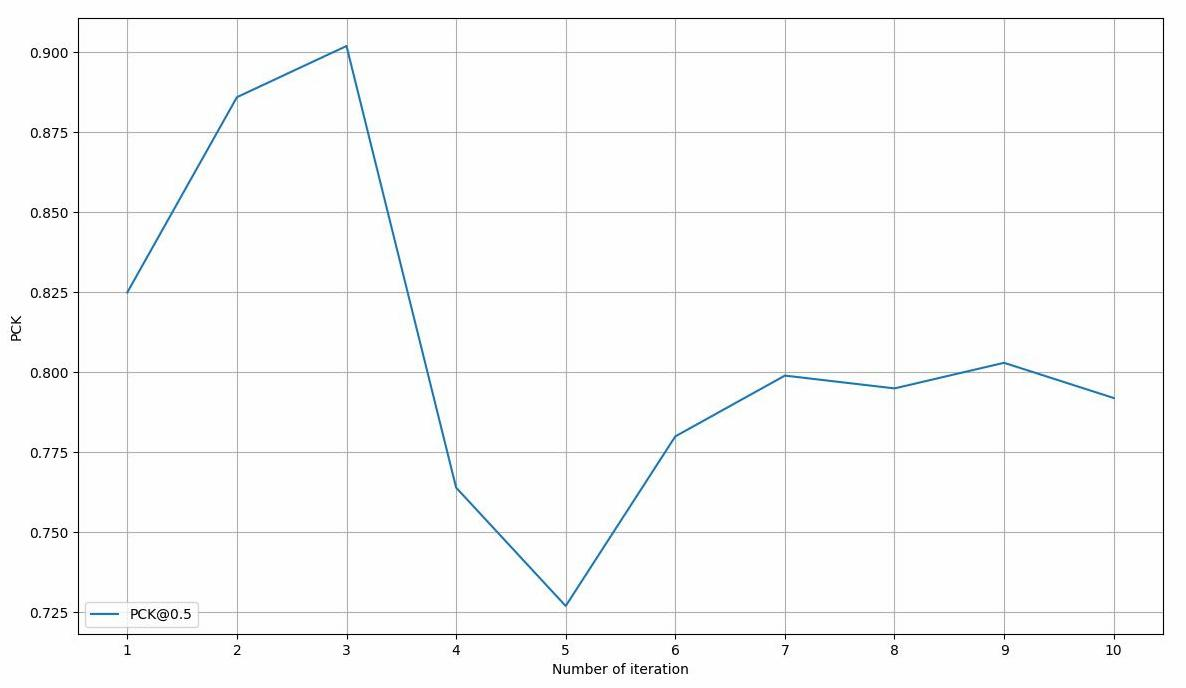
\includegraphics[width=\textwidth]{./images/results/simcc/simcc_pck}
	\caption{PCK@0.5}
	\label{fig:simcc_pck_05}
\end{subfigure}
\begin{subfigure}{.95\textwidth}
	\centering
	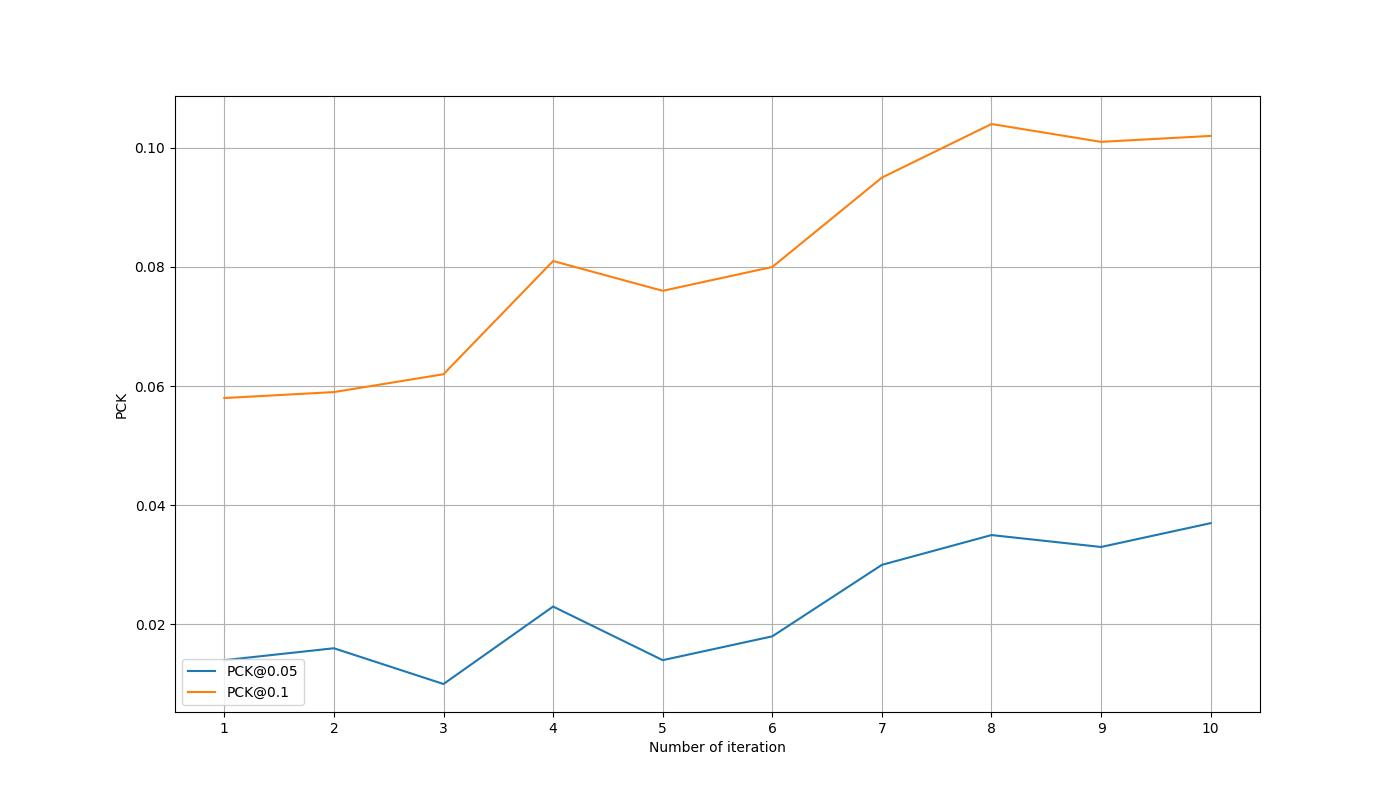
\includegraphics[width=\textwidth]{./images/results/simcc/simcc_pck_small}
	\caption{PCK@0.05 и PCK@0.1}
	\label{fig:simcc_pck_small}
\end{subfigure}
\caption{Зависимость метрики PCK на целевом домене от номера итерации для алгоритма SimCC с магистральной сетью ResNet.}
\label{fig:simcc_pck}
\end{figure}

Данный эксперимент показывает наилучшее качество улучшения результатов предсказаний с помощью алгоритма адаптации. Проигрывает он только дообученной модели в количестве предсказаний с низкой возможной ошибкой. 

Также из \autoref{tab:simcc_table} видно, что дообучение модели не сильно увеличивает количество точек, которые можно считать распознанными. Также видно, что адаптация и дообучение увеличивают высокую точность предсказаний с 1,5 и почти в 3 раза соответственно.

\begin{table}[H]
	\centering
	\begin{tabular}{
	|p{3.3cm}
	||>{\centering\arraybackslash}p{2.2cm}
	|>{\centering\arraybackslash}p{2.2cm}
	|>{\centering\arraybackslash}p{2cm}|}
		\hline
		&PCK@0.05&PCK@0.25&PCK@0.5\\\hline
		\hline
		Baseline & 0.024 & 0.429 & 0.758 \\
		\hline
		Adapted model & 0.037 & 0.445 & 0.792 \\
		\hline
		Finetune model  & 0.062 & 0.411 & 0.76 \\
		\hline
	\end{tabular}
	\begin{tabular}{
	|p{3.3cm}
	||>{\centering\arraybackslash}p{4cm}
	|>{\centering\arraybackslash}p{4.6cm}|}
		\hline
		&Время обучения&Время предсказания\\\hline
		\hline
		Baseline & 80 мин & 83,5 мс\\
		\hline
		Adapted model & 7,75 мин & 82,5 мс\\
		\hline
		Finetune model  & 24 мин & 82,3 мс\\
		\hline
	\end{tabular}
	\caption{Сравнительная статистика нескольких состояний для алгоритма SimCC с магистральной сетью ResNet.}
	\label{tab:simcc_table}
\end{table}

В рамках детального предсказанных точек на \autoref{fig:simcc_distr}, можно заметить, что адаптированная модель очень плохо предсказывает точки глаз, правых запястья и лодыжки. Для метрики в большим трешхолдом (см. \autoref{fig:simcc_distr_05}) в остальных точках адаптированная модель либо показывает наилучшие результаты, либо сопоставимые с базовой моделью. Но для при более точном распознавании (см. \autoref{fig:simcc_distr_025}) заметно ухудшение предсказаний для точеек лица, кроме носа, и плеч.

\begin{figure}[H]
\centering
\begin{subfigure}{.8\textwidth}
	\centering
	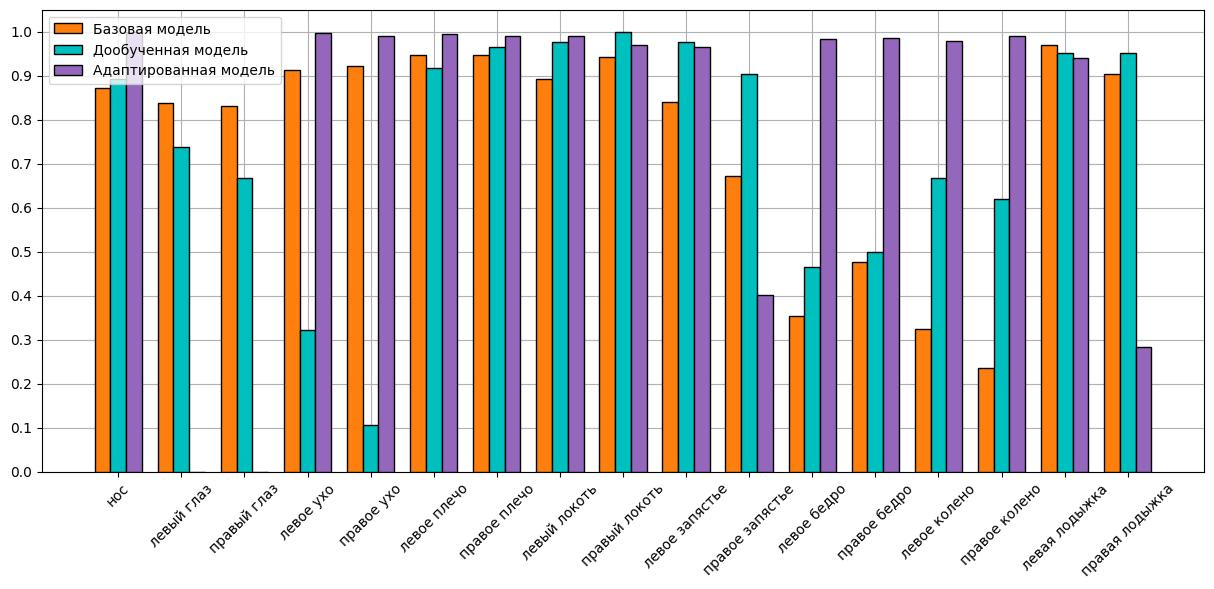
\includegraphics[width=\textwidth]{./images/results/simcc/simcc_05_s}
	\caption{Аналог PCK@0.5}
	\label{fig:simcc_distr_05}
\end{subfigure}
\begin{subfigure}{.8\textwidth}
	\centering
	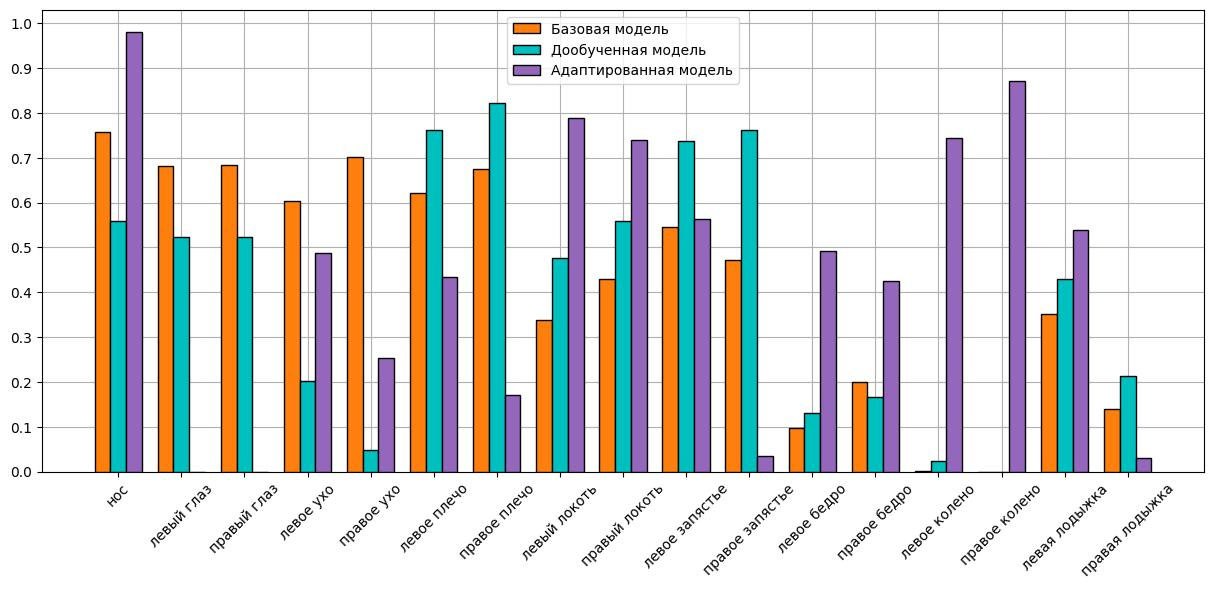
\includegraphics[width=\textwidth]{./images/results/simcc/simcc_025_s}
	\caption{Аналог PCK@0.25}
	\label{fig:simcc_distr_025}
\end{subfigure}
\caption{Распределение корректно предсказанных точек по всей топологии для алгоритма SimCC с магистральной сетью ResNet.}
\label{fig:simcc_distr}
\end{figure}

\subsubsection*{RTMPose}

В рамках последнего эксперимента исследовалась адаптация самой легкой модели. Ее базовая версия показывала наилучшие результаты среди всех исследуемых нейронных сетей. Так как внутри RTMPose реализуется алгоритм SimCC, то ситуация с метриками при итерациях похожая, на предыдущий эксперимент. На \autoref{fig:rtmpose_pck_05} нельяза сказать, что итеративный подход 

\begin{figure}[H]
\centering
\begin{subfigure}{.95\textwidth}
	\centering
	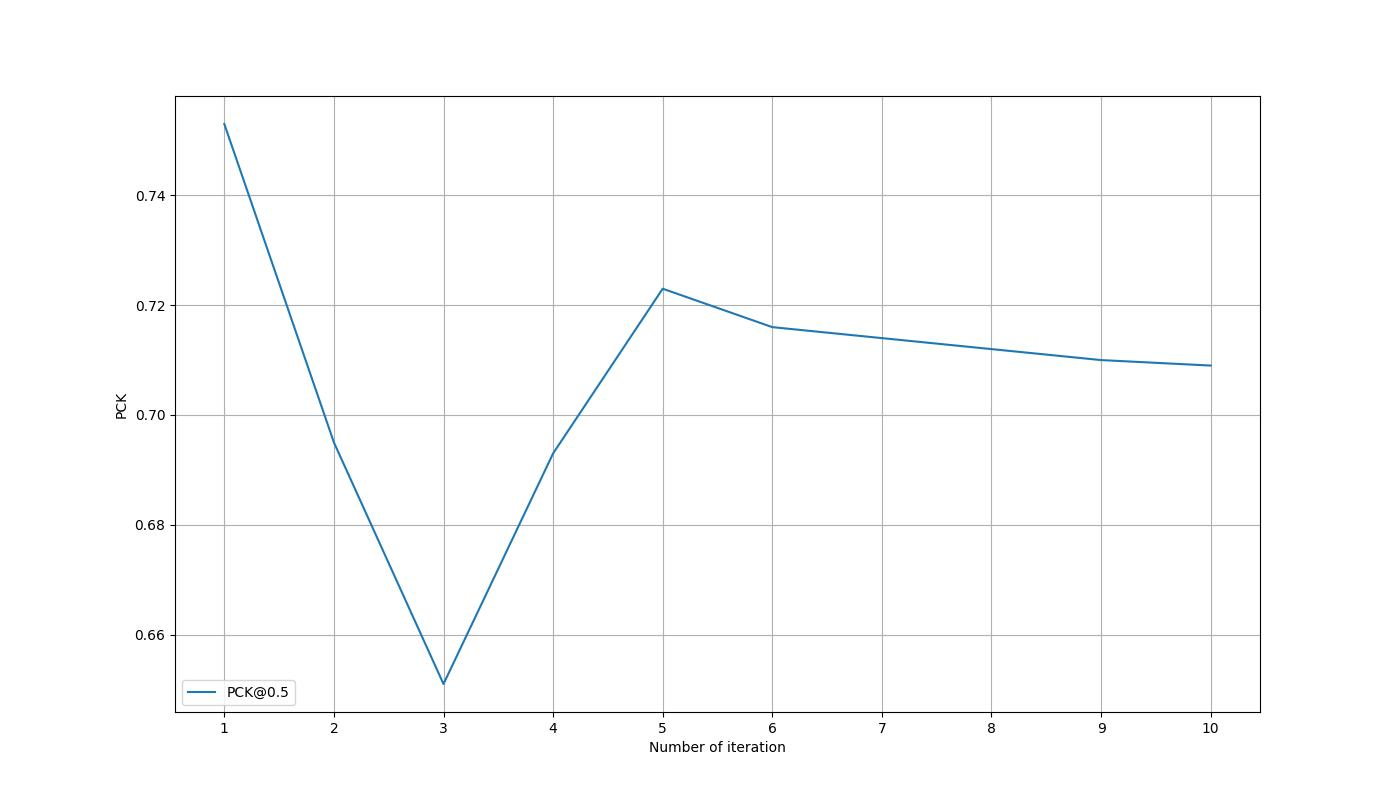
\includegraphics[width=\textwidth]{./images/results/rtmpose/rtmpose_pck}
	\caption{PCK@0.5}
	\label{fig:rtmpose_pck_05}
\end{subfigure}
\begin{subfigure}{.95\textwidth}
	\centering
	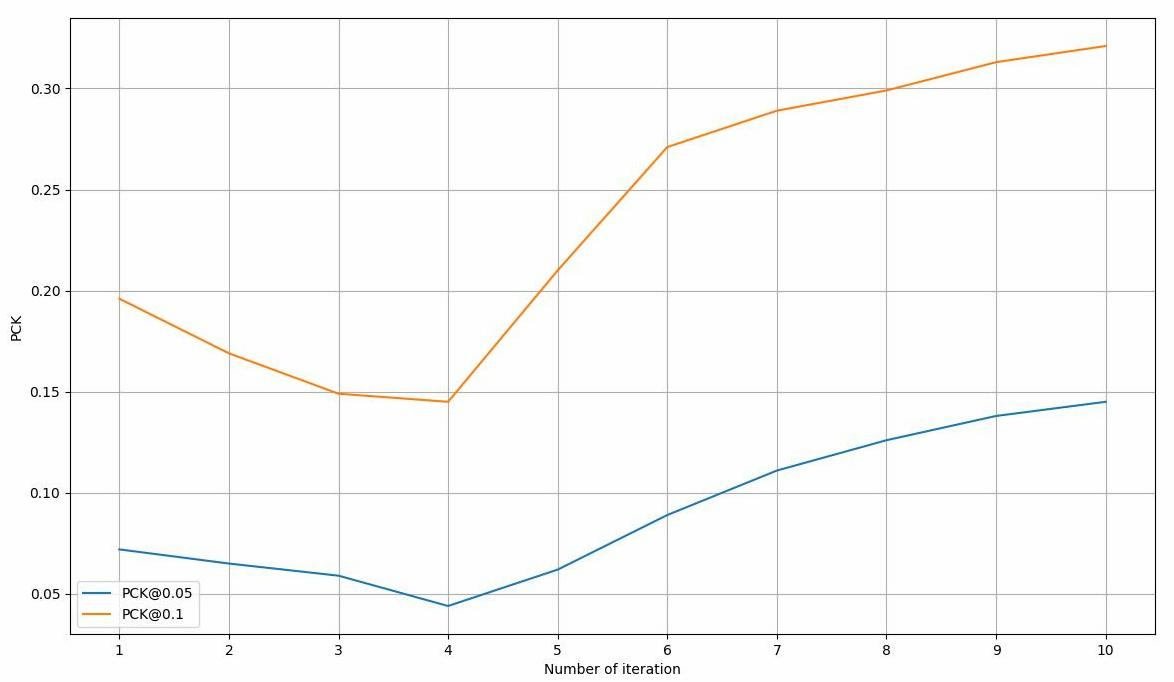
\includegraphics[width=\textwidth]{./images/results/rtmpose/rtmpose_pck_small}
	\caption{PCK@0.05 и PCK@0.1}
	\label{fig:rtmpose_pck_small}
\end{subfigure}
\caption{Зависимость метрики PCK на целевом домене от номера итерации для модели RTMPose.}
\label{fig:rtmpose_pck}
\end{figure}

\begin{table}[H]
	\centering
	\begin{tabular}{
	|p{3.3cm}
	||>{\centering\arraybackslash}p{2.2cm}
	|>{\centering\arraybackslash}p{2.2cm}
	|>{\centering\arraybackslash}p{2cm}|}
		\hline
		&PCK@0.05&PCK@0.25&PCK@0.5\\\hline
		\hline
		Baseline & 0.282 & 0.882 & 0.976 \\
		\hline
		Adapted model & 0.145 & 0.652 & 0.709 \\
		\hline
		Finetune model  & 0.076 & 0.709 & 0.922 \\
		\hline
	\end{tabular}
	\begin{tabular}{
	|p{3.3cm}
	||>{\centering\arraybackslash}p{4cm}
	|>{\centering\arraybackslash}p{4.6cm}|}
		\hline
		&Время обучения&Время предсказания\\\hline
		\hline
		Baseline & 73 мин & 42,4 мс\\
		\hline
		Adapted model & 7,6 мин & 41,7 мс\\
		\hline
		Finetune model  & 22 мин & 41,8 мс\\
		\hline
	\end{tabular}
	\caption{Сравнительная статистика нескольких состояний для модели RTMPose.}
	\label{tab:rtmpose_table}
\end{table}

\begin{figure}[H]
\centering
\begin{subfigure}{.8\textwidth}
	\centering
	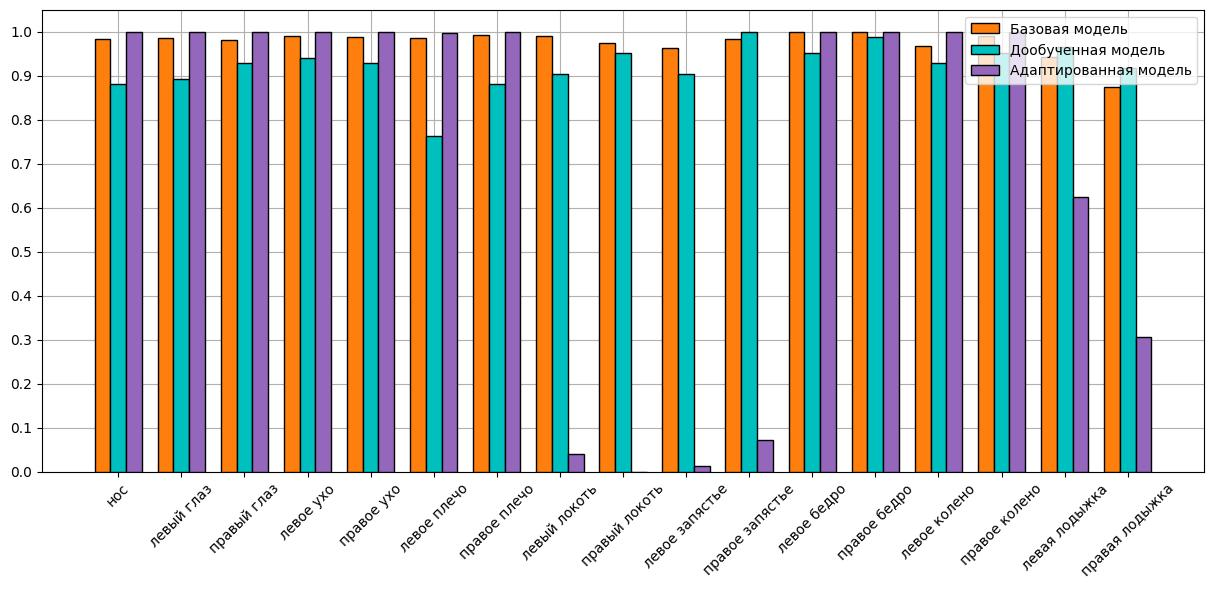
\includegraphics[width=\textwidth]{./images/results/rtmpose/rtmpose_05_s}
	\caption{Аналог PCK@0.5}
	\label{fig:rtmpose_distr_05}
\end{subfigure}
\begin{subfigure}{.8\textwidth}
	\centering
	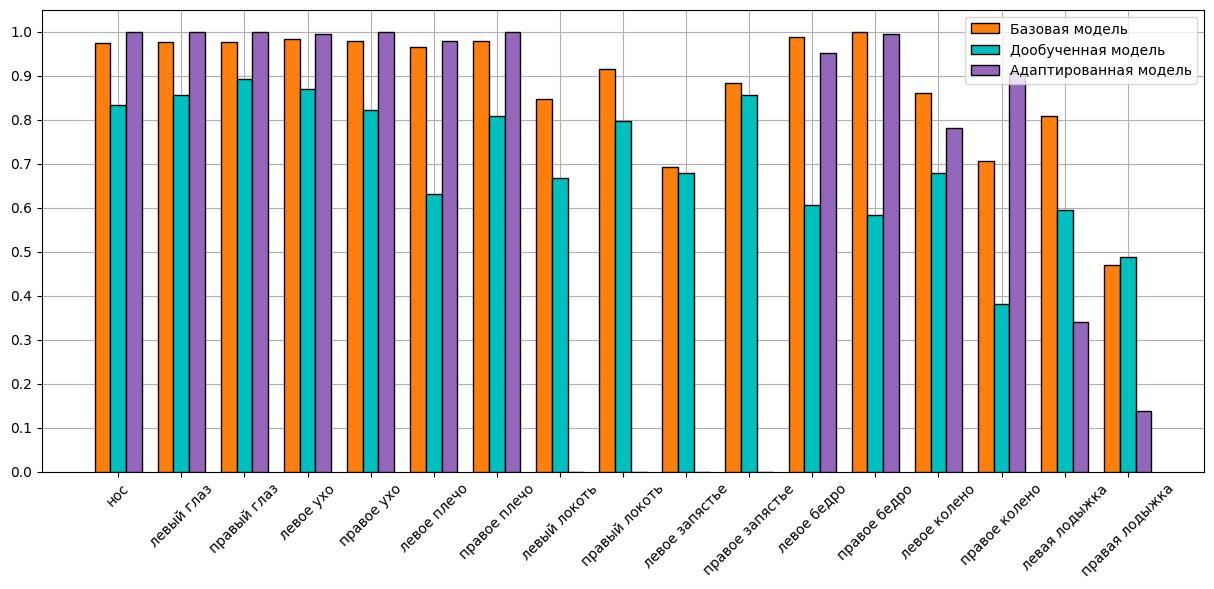
\includegraphics[width=\textwidth]{./images/results/rtmpose/rtmpose_025_s}
	\caption{Аналог PCK@0.25}
	\label{fig:rtmpose_distr_025}
\end{subfigure}
\caption{Распределение корректно предсказанных точек по всей топологии для модели RTMPose.}
\label{fig:rtmpose_distr}
\end{figure}

\newpage